\documentclass[]{article}
\usepackage{lmodern}
\usepackage{amssymb,amsmath}
\usepackage{ifxetex,ifluatex}
\usepackage{fixltx2e} % provides \textsubscript
\ifnum 0\ifxetex 1\fi\ifluatex 1\fi=0 % if pdftex
  \usepackage[T1]{fontenc}
  \usepackage[utf8]{inputenc}
\else % if luatex or xelatex
  \ifxetex
    \usepackage{mathspec}
  \else
    \usepackage{fontspec}
  \fi
  \defaultfontfeatures{Ligatures=TeX,Scale=MatchLowercase}
\fi
% use upquote if available, for straight quotes in verbatim environments
\IfFileExists{upquote.sty}{\usepackage{upquote}}{}
% use microtype if available
\IfFileExists{microtype.sty}{%
\usepackage{microtype}
\UseMicrotypeSet[protrusion]{basicmath} % disable protrusion for tt fonts
}{}
\usepackage[margin=1in]{geometry}
\usepackage{hyperref}
\hypersetup{unicode=true,
            pdftitle={Laborator 6},
            pdfborder={0 0 0},
            breaklinks=true}
\urlstyle{same}  % don't use monospace font for urls
\usepackage{natbib}
\bibliographystyle{plainnat}
\usepackage{color}
\usepackage{fancyvrb}
\newcommand{\VerbBar}{|}
\newcommand{\VERB}{\Verb[commandchars=\\\{\}]}
\DefineVerbatimEnvironment{Highlighting}{Verbatim}{commandchars=\\\{\}}
% Add ',fontsize=\small' for more characters per line
\usepackage{framed}
\definecolor{shadecolor}{RGB}{248,248,248}
\newenvironment{Shaded}{\begin{snugshade}}{\end{snugshade}}
\newcommand{\KeywordTok}[1]{\textcolor[rgb]{0.13,0.29,0.53}{\textbf{#1}}}
\newcommand{\DataTypeTok}[1]{\textcolor[rgb]{0.13,0.29,0.53}{#1}}
\newcommand{\DecValTok}[1]{\textcolor[rgb]{0.00,0.00,0.81}{#1}}
\newcommand{\BaseNTok}[1]{\textcolor[rgb]{0.00,0.00,0.81}{#1}}
\newcommand{\FloatTok}[1]{\textcolor[rgb]{0.00,0.00,0.81}{#1}}
\newcommand{\ConstantTok}[1]{\textcolor[rgb]{0.00,0.00,0.00}{#1}}
\newcommand{\CharTok}[1]{\textcolor[rgb]{0.31,0.60,0.02}{#1}}
\newcommand{\SpecialCharTok}[1]{\textcolor[rgb]{0.00,0.00,0.00}{#1}}
\newcommand{\StringTok}[1]{\textcolor[rgb]{0.31,0.60,0.02}{#1}}
\newcommand{\VerbatimStringTok}[1]{\textcolor[rgb]{0.31,0.60,0.02}{#1}}
\newcommand{\SpecialStringTok}[1]{\textcolor[rgb]{0.31,0.60,0.02}{#1}}
\newcommand{\ImportTok}[1]{#1}
\newcommand{\CommentTok}[1]{\textcolor[rgb]{0.56,0.35,0.01}{\textit{#1}}}
\newcommand{\DocumentationTok}[1]{\textcolor[rgb]{0.56,0.35,0.01}{\textbf{\textit{#1}}}}
\newcommand{\AnnotationTok}[1]{\textcolor[rgb]{0.56,0.35,0.01}{\textbf{\textit{#1}}}}
\newcommand{\CommentVarTok}[1]{\textcolor[rgb]{0.56,0.35,0.01}{\textbf{\textit{#1}}}}
\newcommand{\OtherTok}[1]{\textcolor[rgb]{0.56,0.35,0.01}{#1}}
\newcommand{\FunctionTok}[1]{\textcolor[rgb]{0.00,0.00,0.00}{#1}}
\newcommand{\VariableTok}[1]{\textcolor[rgb]{0.00,0.00,0.00}{#1}}
\newcommand{\ControlFlowTok}[1]{\textcolor[rgb]{0.13,0.29,0.53}{\textbf{#1}}}
\newcommand{\OperatorTok}[1]{\textcolor[rgb]{0.81,0.36,0.00}{\textbf{#1}}}
\newcommand{\BuiltInTok}[1]{#1}
\newcommand{\ExtensionTok}[1]{#1}
\newcommand{\PreprocessorTok}[1]{\textcolor[rgb]{0.56,0.35,0.01}{\textit{#1}}}
\newcommand{\AttributeTok}[1]{\textcolor[rgb]{0.77,0.63,0.00}{#1}}
\newcommand{\RegionMarkerTok}[1]{#1}
\newcommand{\InformationTok}[1]{\textcolor[rgb]{0.56,0.35,0.01}{\textbf{\textit{#1}}}}
\newcommand{\WarningTok}[1]{\textcolor[rgb]{0.56,0.35,0.01}{\textbf{\textit{#1}}}}
\newcommand{\AlertTok}[1]{\textcolor[rgb]{0.94,0.16,0.16}{#1}}
\newcommand{\ErrorTok}[1]{\textcolor[rgb]{0.64,0.00,0.00}{\textbf{#1}}}
\newcommand{\NormalTok}[1]{#1}
\usepackage{longtable,booktabs}
\usepackage{graphicx,grffile}
\makeatletter
\def\maxwidth{\ifdim\Gin@nat@width>\linewidth\linewidth\else\Gin@nat@width\fi}
\def\maxheight{\ifdim\Gin@nat@height>\textheight\textheight\else\Gin@nat@height\fi}
\makeatother
% Scale images if necessary, so that they will not overflow the page
% margins by default, and it is still possible to overwrite the defaults
% using explicit options in \includegraphics[width, height, ...]{}
\setkeys{Gin}{width=\maxwidth,height=\maxheight,keepaspectratio}
\IfFileExists{parskip.sty}{%
\usepackage{parskip}
}{% else
\setlength{\parindent}{0pt}
\setlength{\parskip}{6pt plus 2pt minus 1pt}
}
\setlength{\emergencystretch}{3em}  % prevent overfull lines
\providecommand{\tightlist}{%
  \setlength{\itemsep}{0pt}\setlength{\parskip}{0pt}}
\setcounter{secnumdepth}{5}
% Redefines (sub)paragraphs to behave more like sections
\ifx\paragraph\undefined\else
\let\oldparagraph\paragraph
\renewcommand{\paragraph}[1]{\oldparagraph{#1}\mbox{}}
\fi
\ifx\subparagraph\undefined\else
\let\oldsubparagraph\subparagraph
\renewcommand{\subparagraph}[1]{\oldsubparagraph{#1}\mbox{}}
\fi

%%% Use protect on footnotes to avoid problems with footnotes in titles
\let\rmarkdownfootnote\footnote%
\def\footnote{\protect\rmarkdownfootnote}

%%% Change title format to be more compact
\usepackage{titling}

% Create subtitle command for use in maketitle
\newcommand{\subtitle}[1]{
  \posttitle{
    \begin{center}\large#1\end{center}
    }
}

\setlength{\droptitle}{-2em}
  \title{Laborator 6}
  \pretitle{\vspace{\droptitle}\centering\huge}
  \posttitle{\par}
\subtitle{Elemente de regresie liniară multiplă}
  \author{}
  \preauthor{}\postauthor{}
  \date{}
  \predate{}\postdate{}

\usepackage{booktabs}
\usepackage{longtable}
\usepackage{framed,color}
\definecolor{shadecolor}{RGB}{248, 248, 248}
%\definecolor{shadecolor1}{RGB}{216,225,235}
%\definecolor{framecolor}{RGB}{108,123,13}

%\definecolor{shadecolor}{RGB}{226, 255, 241}
\definecolor{shadecolor1}{RGB}{217,225,199}
\definecolor{framecolor}{RGB}{60,179,113}

%%%%%%%%%%%%%%%%%%%%%%
\ifxetex
  \usepackage{letltxmacro}
  \setlength{\XeTeXLinkMargin}{1pt}
  \LetLtxMacro\SavedIncludeGraphics\includegraphics
  \def\includegraphics#1#{% #1 catches optional stuff (star/opt. arg.)
    \IncludeGraphicsAux{#1}%
  }%
  \newcommand*{\IncludeGraphicsAux}[2]{%
    \XeTeXLinkBox{%
      \SavedIncludeGraphics#1{#2}%
    }%
  }%
\fi

\newenvironment{frshaded*}{%
  \def\FrameCommand{\fboxrule=\FrameRule\fboxsep=\FrameSep \fcolorbox{framecolor}{shadecolor1}}%
  \MakeFramed {\advance\hsize-\width \FrameRestore}}%
{\endMakeFramed}

\newenvironment{rmdblock}[1]
  {\begin{frshaded*}
  \begin{itemize}
  \renewcommand{\labelitemi}{
    \raisebox{-.7\height}[0pt][0pt]{
      {\setkeys{Gin}{width=2em,keepaspectratio}\includegraphics{images/icons/#1}}
    }
  }
  \item
  }
  {
  \end{itemize}
  \end{frshaded*}
  }
  
%%%%%%%%%%%%%%%
% definitions.
% -------------------
\usepackage{marginnote}
% \renewcommand*{\marginnotevadjust}{40pt}
% \renewcommand{\marginnotevadjust}{0pt}
% \renewcommand{\marginfont}{\noindent\rule{0pt}{0.7\baselineskip}\tiny}

\newtheorem{proposition}{Proposition}[section]
\newtheorem{lemma}[proposition]{Lemma}
\newtheorem{corollary}[proposition]{Corollary}
\newtheorem{theorem}[proposition]{Theorem}

\newcounter{exo}[section]
\newcommand{\enonce}[2]{\refstepcounter{proposition}\hypertarget{exo:#1}{}\label{exo:#1}{\scriptsize\;\textbf{Ex.}~\ref{exo:#1}}}

\reversemarginpar
\setlength{\marginparwidth}{1.2cm}
% 
% \newcommand{\enonce}[2]{\refstepcounter{proposition}\hypertarget{exo:#1}{}\label{exo:#1}{\noindent\color{black}\normalsize\bf Exercice \ref{exo:#1}}\ \  #2\vspace{1mm}\hrule\vspace{1mm} \color{black}\normalsize}


%%%%%%%%%%%%%%%

\newenvironment{rmdcaution}
  {\begin{rmdblock}{caution}}
  {\end{rmdblock}}
% \newenvironment{rmdinsight}
%   {\begin{rmdblock}{insight}}
%   {\end{rmdblock}}

\newenvironment{rmdexercise}
  {\begin{rmdblock}{exercise}}
  {\end{rmdblock}}

% \newenvironment{rmdexercise_tex}
%   {\begin{rmdblock}{exercise}}
%   {\end{rmdblock}}
  
\newenvironment{rmdtip}
  {\begin{rmdblock}{tip}}
  {\end{rmdblock}}


%%%%%%%%%%%%%%%%%%%%%%%%%%%%%%%%%%%%%%%%%%%%%%%%%%%%%%%%%%%%%%%%%%%%%%%%%%%%%%%%%%%%%%%%%%%%%%%%%%%%%%%%%%%%%%%%%%%%%
%%%%%%%%%%% For insight block %%%%%%%%%%%%%%%%%%%%%%%%%%
\definecolor{shadecolor_insight}{RGB}{223,240,216}
\definecolor{framecolor_insight}{RGB}{136,193,137}

%\definecolor{shadecolor_insight}{RGB}{217,225,199}
%\definecolor{framecolor_insight}{RGB}{60,179,113}

\newenvironment{frshaded_insight*}{%
  \def\FrameCommand{\fboxrule=\FrameRule\fboxsep=\FrameSep \fcolorbox{framecolor_insight}{shadecolor_insight}}%
  \MakeFramed {\advance\hsize-\width \FrameRestore}}%
{\endMakeFramed}

\newenvironment{rmdblock_insight}[1]
  {\begin{frshaded_insight*}
  \begin{itemize}
  \renewcommand{\labelitemi}{
    \raisebox{-.7\height}[0pt][0pt]{
      {\setkeys{Gin}{width=2em,keepaspectratio}\includegraphics{images/icons/#1}}
    }
  }
  \item
  }
  {
  \end{itemize}
  \end{frshaded_insight*}
  }

\newenvironment{rmdinsight}
  {\begin{rmdblock_insight}{insight}}
  {\end{rmdblock_insight}}

%%%%%%%%%%%%%%%%%%%%%%%%%%%%%%%%%%%%%%%%%%%%%%%%%%%%%%%%%%%%%%%%%%%%%%%%%%%%%%%%%%%%%%%%%%%%%%%%%%%%%%%%%%%%%%%%%%%%%
\usepackage{subfigure}
\usepackage{booktabs}
\usepackage{slashbox}
\usepackage{color}
%%%%%%%%%%%%%%%%%%%%%%%%%%%%%%%%%%%%%%%%%
\definecolor{linkcol}{rgb}{0,0,0.4}
\definecolor{citecol}{rgb}{0.5,0,0}

% Change this to change the informations included in the pdf file
% \usepackage[pagebackref]{hyperref}
% \usepackage[verbose]{backref}
\usepackage[hyperpageref]{backref}
% \backrefsetup{verbose=false}
% \PassOptionsToPackage{pagebackref}{hyperref}
% See hyperref documentation for information on those parameters

\hypersetup
{
bookmarksopen=true,
pdftitle="Curs Instrumente Statistice pentru Finante",
pdfauthor="Alexandru Amarioarei",
pdfsubject="Laboratoare Instrumente Statistice pentru Finante", %subject of the document
pdfmenubar=true, %menubar shown
pdfhighlight=/O, %effect of clicking on a link
colorlinks=true, %couleurs sur les liens hypertextes
pdfpagemode=None, %aucun mode de page
pdfpagelayout=SinglePage, %ouverture en simple page
pdffitwindow=true, %pages ouvertes entierement dans toute la fenetre
linkcolor=linkcol, %couleur des liens hypertextes internes
citecolor=citecol, %couleur des liens pour les citations
urlcolor=linkcol %couleur des liens pour les url
}


% set the back references
\renewcommand*{\backref}[1]{}
\renewcommand*{\backreftwosep}{ și~} % inserted between entries 
                              % in a list of two entries, 
                              % default is " and~".
\renewcommand*{\backreflastsep}{ și~} % inserted between the last 
                               % two entries of a list with more
                               % than two entries, default is ", and~".
\renewcommand*{\backrefalt}[4]{%
    \ifcase #1 (Necitat.)%
    \or        (Citat la pagina~#2.)%
    \else      (Citat la paginile~#2.)%
    \fi}

%%%%%%%%%%%%%%%%%%%%%%%%%%%%%%%%%%%%%%%%%%%%%%%%%%%%%%%%%%%%%%%%%%%%%%%%%%%%%%%%%%%%%%%%%%%%%%%%%%%%%%%%%%%%%%%%%%%%%
%CITEVA DEFINITII
\def\om{\omega}
\def\Om{\Omega}
\def\et{\eta}
\def\td{\tilde{\delta}}
\def\m{{\mu}}
\def\n{{\nu}}
\def\k{{\kappa}}
\def\l{{\lambda}}
\def\L{{\Lambda}}
\def\g{{\gamma}}
\def\a{{\alpha}}
\def\e{{\varepsilon}}
\def\b{{\beta}}
\def\G{{\Gamma}}
\def\d{{\delta}}
\def\D{{\Delta}}
\def\t{{\theta}}
\def\s{{\sigma}}
\def\S{{\Sigma}}
\def\z{{\zeta}}
\def\qed{\hfill\Box}
\def\ds{\displaystyle}
\def\mc{\mathcal}
%%%%%%%%%%%%%%%%%%%%%%%%%%%%%%%%%%%%%%%%%%%%%%%%%%%%%%%%%%%%%%%%%%%%%%%%%%%%%%%%%%%%%%%%%%%%%%%%%%%%%%%%%%%%%%%%%%%%%%
\def\1{{\mathbf 1}}
\def\CC{{\mathbb C}}
\def\VV{{\mathbb V}}
\def\RR{{\mathbb R}}
\def\QQ{{\mathbb Q}}
\def\ZZ{{\mathbb Z}}
\def\PP{{\mathbb P}}
\def\EE{{\mathbb E}}
\def\NN{{\mathbb N}}
\def\FF{{\mathbb F}}
%\def\SS{{\mathbb S}}
\def\MA{{\mathcal A}}
\def\MO{{\mathcal O}}
\def\MF{{\mathcal F}}
\def\ME{{\mathcal E}}
\def\MR{{\mathcal R}}
\def\MB{{\mathcal B}}
\def\MM{{\mathcal M}}
\def\MN{{\mathcal N}}
\def\MU{{\mathcal U}}
\def\MP{{\mathcal P}}
\def\MS{{\mathcal S}}
\def\MBS{{\mathbf S}}
\def\MX{{\bm{ \mathscr X}}}

% independent sign
\newcommand\independent{\protect\mathpalette{\protect\independenT}{\perp}}
\def\independenT#1#2{\mathrel{\rlap{$#1#2$}\mkern2mu{#1#2}}}

\renewcommand\tablename{Tab.}
\renewcommand{\figurename}{Fig.}
\renewcommand\refname{Referințe}

%%%%%%%%%%%%%%%%%%%%%%%%%%%%%%%%%%%%%%%%%%%%%%%%%%%%%%%%%%%%%%%%%%%%%%%%%%%%%%%%%%%%%%%%%%%%%%%%%%%%%%%%%%%%%%%%%%%%%
%Header and Footer
\usepackage{fancyhdr}

\pagestyle{fancy}
\fancyhf{}
\rhead{Universitatea din Bucure\c sti\\ Facultatea de Matematic\u a \c si Informatic\u a}
\lhead{\textit{Curs}: Instrumente Statistice pentru Finan\c te\\ \textit{Instructor}: A. Am\u arioarei}
\rfoot{Pagina \thepage}
\lfoot{Grupa: 403}
%%%%%%%%%%%%%%%%%%%%%%%%%%%%%%%%%%%%%%%
\usepackage{booktabs}
\usepackage{longtable}
\usepackage{array}
\usepackage{multirow}
\usepackage[table]{xcolor}
\usepackage{wrapfig}
\usepackage{float}
\usepackage{colortbl}
\usepackage{pdflscape}
\usepackage{tabu}
\usepackage{threeparttable}
\usepackage{threeparttablex}
\usepackage[normalem]{ulem}
\usepackage{makecell}

\begin{document}
\maketitle

%%%%%%%%%%%%%%%%%%%%%%%%
\thispagestyle{fancy}

Obiectivul acestui laborator este de a prezenta câteva exemple legate de
problema de regresie liniară simplă.

\section{Introducere}\label{introducere}

Modelul de regresie liniară multiplă reprezintă o generalizare a
modelului de regresie simplă. Dacă în regresia liniară simplă se folosea
o singură variabilă predictor \(X\) ca să explice variabila răspuns
\(Y\), în modelul de regresie liniară multiplă se folosesc mai multe
variabile predictor \(X_1,\ldots,X_k\) pentru a explica răspunsul \(Y\):

\[
\mathbb{E}[Y|X_1 = x_1, \ldots, X_k=x_x]=\beta_0+\beta_1x_1+\beta_2x_2+\ldots+\beta_kx_k
\] sau altfel scris

\[
Y = \beta_0 + \beta_1 X_1 + \ldots + \beta_k X_k + \varepsilon.
\]

Date fiind observațiile actuale, cu alte cuvinte dat fiind un eșantion
\((X_{11},\ldots,X_{1k},Y_1),\ldots,(X_{n1},\ldots,X_{nk},Y_n)\) al lui
\((X_1,\ldots,X_k,Y)\), unde \(X_{ij}\) reprezintă a \(i\)-a observație
a predictorului \(X_j\), modelul se poate scrie

\[
y_i = \beta_0+\beta_1x_{i1}+\beta_2x_{i2}+\ldots+\beta_kx_{ik}+\varepsilon_i, \quad i = 1,\ldots,n
\]

a cărui formă compactă (matriceală) este

\[
\mathbf{Y}=\mathbf{X}\boldsymbol\beta+\boldsymbol\varepsilon
\]

\begin{itemize}
\tightlist
\item
  \(\mathbf{X}\) este \emph{matricea de design}
\end{itemize}

\[
\mathbf{X}=\begin{pmatrix}
1 & X_{11} & \cdots & X_{1k}\\
\vdots & \vdots & \ddots & \vdots\\
1 & X_{n1} & \cdots & X_{nk}
\end{pmatrix}_{n\times(k+1)}
\]

\begin{itemize}
\tightlist
\item
  \(\mathbf{Y}\) este \emph{vectorul răspuns}, \(\boldsymbol\beta\) este
  \emph{vectorul coeficienților} iar \(\boldsymbol\varepsilon\) este
  \emph{vectorul eroare}
\end{itemize}

\[
\mathbf{Y}=\begin{pmatrix}
Y_1 \\
\vdots \\
Y_n
\end{pmatrix}_{n\times 1},\quad\boldsymbol\beta=\begin{pmatrix}
\beta_0 \\
\beta_1 \\
\vdots \\
\beta_k
\end{pmatrix}_{(k+1)\times 1}\text{ și }\quad
\boldsymbol\varepsilon=\begin{pmatrix}
\varepsilon_1 \\
\vdots \\
\varepsilon_n
\end{pmatrix}_{n\times 1}.
\]

\begin{rmdinsight}
Să observăm că pentru \(k=1\) modelul se reduce la regresia liniară
simplă. În acest caz:

\[
\mathbf{X}=\begin{pmatrix}
1 & X_{11}\\
\vdots & \vdots\\
1 & X_{n1}
\end{pmatrix}_{n\times2}\text{ și }\quad \beta=\begin{pmatrix}
\beta_0 \\
\beta_1 
\end{pmatrix}_{2\times 1}
\]
\end{rmdinsight}

\emph{Suma abaterilor pătratice reziduale} pentru modelul de regresie
liniară multiplă este

\[
RSS(\boldsymbol\beta)=\sum_{i=1}^n(Y_i-\beta_0-\beta_1X_{i1}-\ldots-\beta_kX_{ik})^2=(\mathbf{Y}-\mathbf{X}\boldsymbol{\beta})^T(\mathbf{Y}-\mathbf{X}\boldsymbol{\beta})
\]

ceea ce conduce la \emph{sistemul de ecuații normale}

\[
\mathbf{X}^\intercal\mathbf{X}\hat{\boldsymbol{\beta}}=\mathbf{X}^\intercal\mathbf{Y}
\]

a cărui soluție, dat fiind că \(\mathbf{X}^\intercal\mathbf{X}\) este
inversabilă, este

\[
\hat{\boldsymbol{\beta}}=(\mathbf{X}^\intercal\mathbf{X})^{-1}\mathbf{X}^\intercal\mathbf{Y}
\]

Odată ce avem estimatorul \(\hat{\boldsymbol{\beta}}\), putem defini:

\begin{itemize}
\tightlist
\item
  \emph{valorile prognozate} (\emph{fitted values})
  \(\hat Y_1,\ldots,\hat Y_n\) (valorile verticale pe hiperplanul de
  regresie), unde
\end{itemize}

\[
\hat Y_i=\hat\beta_0+\hat\beta_1X_{i1}+\cdots+\hat\beta_kX_{ik},\quad i=1,\ldots,n
\]

și sub formă matriceală

\[
\hat{\mathbf{Y}}=\mathbf{X}\hat{\boldsymbol{\beta}}=\mathbf{X}(\mathbf{X}^\intercal\mathbf{X})^{-1}\mathbf{X}^\intercal\mathbf{Y}=\mathbf{H}\mathbf{Y}
\]

unde
\(\mathbf{H}=\mathbf{X}(\mathbf{X}^\intercal\mathbf{X})^{-1}\mathbf{X}^\intercal\)
se numește \emph{matricea căciulă} (\emph{hat matrix}) și reprezintă
proiecția ortogonală a lui \(\mathbf{Y}\) în spațiul generat de
\(\mathbf{X}\).

\begin{itemize}
\tightlist
\item
  \emph{reziduurile estimate} (\emph{estimated residuals})
  \(\hat \varepsilon_1,\ldots,\hat \varepsilon_n\), unde
\end{itemize}

\[
\hat\varepsilon_i=Y_i-\hat Y_i,\quad i=1,\ldots,n
\]

și sub formă matriceală

\[
\hat{\boldsymbol\varepsilon} = \boldsymbol Y - \hat{\boldsymbol Y} = (\boldsymbol I-\boldsymbol H)\boldsymbol Y
\]

În figura de mai jos ilustrăm planul de regresie (albastru) și relația
cu regresiile liniare simple (liniile verzi). Punctele roșii reprezintă
un eșantion pentru \((X_1,X_2,Y)\) iar punctele negre sunt subeșantioane
pentru \((X_1,X_2)\) (la bază), \((X_1,Y)\) (stânga) și \((X_2,Y)\)
(dreapta).

\begin{center}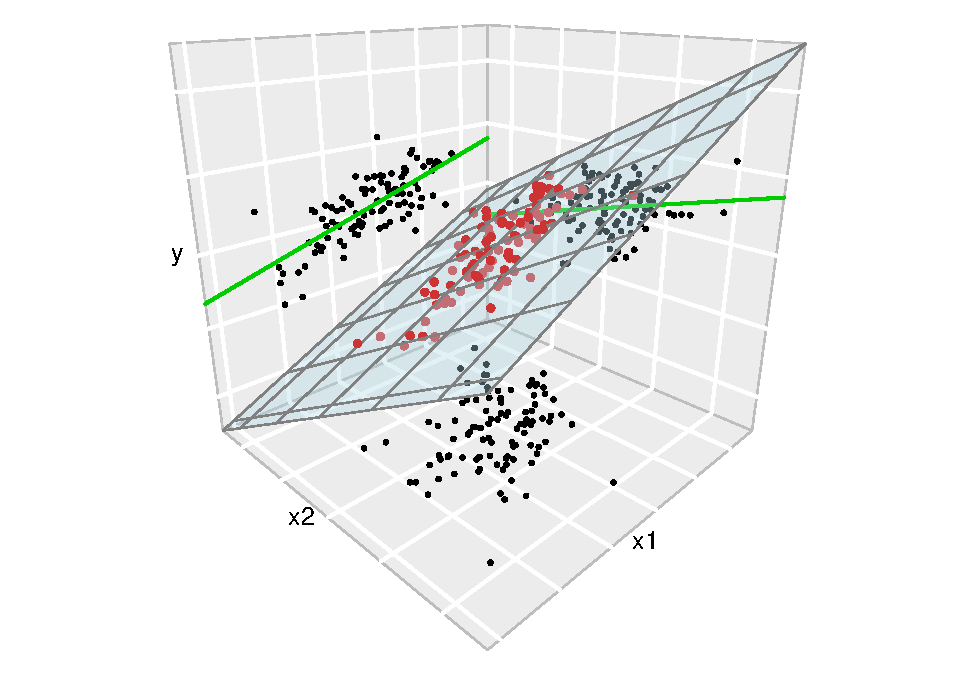
\includegraphics[width=0.7\linewidth]{Lab_6_files/figure-latex/unnamed-chunk-4-1} \end{center}

Ipotezele modelului sunt:

\begin{enumerate}
\def\labelenumi{\roman{enumi}.}
\tightlist
\item
  \textbf{Linearitatea}:
  \(\mathbb{E}[Y|X_1=x_1,\ldots,X_k=x_k]=\beta_0+\beta_1x_1+\ldots+\beta_kx_k\)
\item
  \textbf{Homoscedasticitatea}:
  \(\mathbb{V}\text{ar}(\varepsilon_i)=\sigma^2\), cu \(\sigma^2\)
  constantă pentru \(i=1,\ldots,n\)
\item
  \textbf{Normalitatea}: \(\varepsilon_i\sim\mathcal{N}(0,\sigma^2)\)
  pentru \(i=1,\ldots,n\)
\item
  \textbf{Independența erorilor}: \(\varepsilon_1,\ldots,\varepsilon_n\)
  sunt independente (sau necorelate,
  \(\mathbb{E}[\varepsilon_i\varepsilon_j]=0\), \(i\neq j\), deoarece
  sunt presupuse normale)
\end{enumerate}

Altfel spus

\[
Y|(X_1=x_1,\ldots,X_k=x_k)\sim \mathcal{N}(\beta_0+\beta_1x_1+\ldots+\beta_kx_k,\sigma^2)
\]

În figura de mai jos afișam planul de regresie. Spațiul dintre cele două
plane galbene arată unde se află 95\% din observații (după modelul
ales).

\begin{center}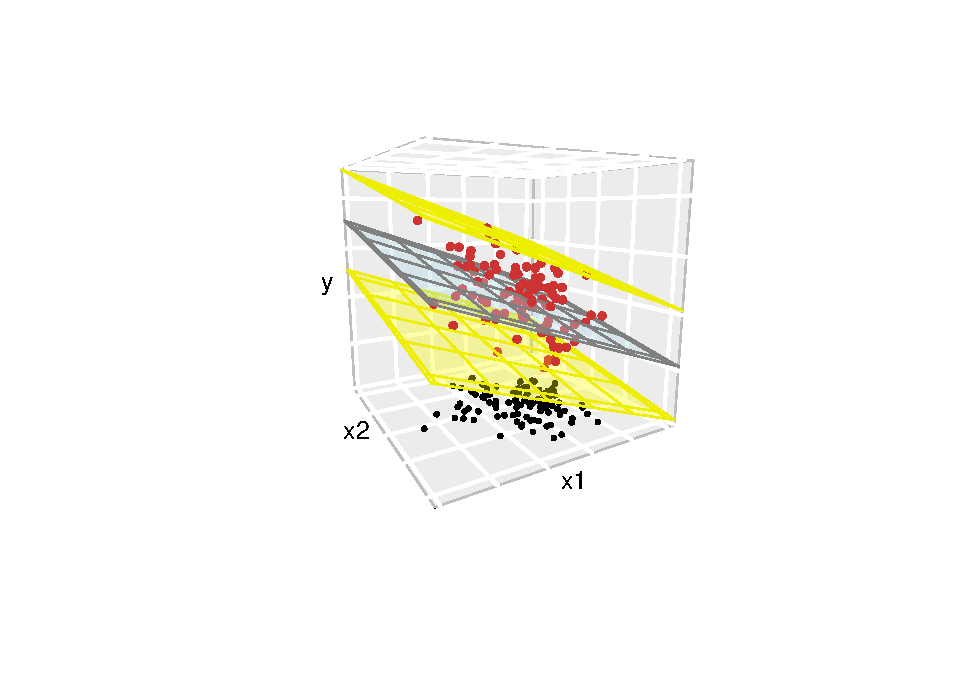
\includegraphics[width=0.7\linewidth]{Lab_6_files/figure-latex/unnamed-chunk-5-1} \end{center}

Estimatorul pentru \(\sigma^2\) este

\[
\hat{\sigma}^2 = \frac{RSS(\hat{\beta}_0,\hat{\beta}_1,\ldots, \hat{\beta}_k))}{n-(k+1)} = \frac{\hat{\boldsymbol \varepsilon}^\intercal\hat{\boldsymbol \varepsilon}}{n-(k+1)} = \frac{\sum_{i=1}^{n}\hat{\varepsilon}_i^2}{n-(k+1)}.
\]

\section{Aplicație}\label{aplicatie}

Această aplicație este bazată pe articolul \citep{Johnson1973}.

\begin{rmdexercise}
Considerăm setul de date \href{dataIn/galapagos.csv}{galapagos} care
conține informații despre numărul de specii de broaște țestoase din
diferite insule din arhipelagul Galapagos. Setul conține date din 30 de
insule despre numărul de specii de țestoase (\texttt{Species}), numărul
de specii endemice (\texttt{Endemics}), suprafața insulei
(\texttt{Area}), înălțimea maximă a insulei (`\texttt{Elevation}),
distanța la cea mai apropiată insulă (\texttt{Nearest}), distanța față
de insula Snata Cruz (\texttt{Scruz}) și suprafața insulei adiacente
(\texttt{Adjacent}). Vrem să investigăm relația liniară dintre numărul
de specii și celelalte variabile.
\end{rmdexercise}

Începem prin a citi datele

\begin{Shaded}
\begin{Highlighting}[]
\CommentTok{# gala = read.csv("data/galapagos.csv", row.names = 1)}

\KeywordTok{data}\NormalTok{(}\StringTok{"gala"}\NormalTok{) }\CommentTok{# este nevoie de libraria faraway}
\KeywordTok{head}\NormalTok{(gala)}
\NormalTok{             Species Endemics  Area Elevation Nearest Scruz Adjacent}
\NormalTok{Baltra            }\DecValTok{58}       \DecValTok{23} \FloatTok{25.09}       \DecValTok{346}     \FloatTok{0.6}   \FloatTok{0.6}     \FloatTok{1.84}
\NormalTok{Bartolome         }\DecValTok{31}       \DecValTok{21}  \FloatTok{1.24}       \DecValTok{109}     \FloatTok{0.6}  \FloatTok{26.3}   \FloatTok{572.33}
\NormalTok{Caldwell           }\DecValTok{3}        \DecValTok{3}  \FloatTok{0.21}       \DecValTok{114}     \FloatTok{2.8}  \FloatTok{58.7}     \FloatTok{0.78}
\NormalTok{Champion          }\DecValTok{25}        \DecValTok{9}  \FloatTok{0.10}        \DecValTok{46}     \FloatTok{1.9}  \FloatTok{47.4}     \FloatTok{0.18}
\NormalTok{Coamano            }\DecValTok{2}        \DecValTok{1}  \FloatTok{0.05}        \DecValTok{77}     \FloatTok{1.9}   \FloatTok{1.9}   \FloatTok{903.82}
\NormalTok{Daphne.Major      }\DecValTok{18}       \DecValTok{11}  \FloatTok{0.34}       \DecValTok{119}     \FloatTok{8.0}   \FloatTok{8.0}     \FloatTok{1.84}
\end{Highlighting}
\end{Shaded}

Considerăm modelul de regresie liniară multiplă cu 5 predictori:

\begin{Shaded}
\begin{Highlighting}[]
\NormalTok{gala_model =}\StringTok{ }\KeywordTok{lm}\NormalTok{(Species }\OperatorTok{~}\StringTok{ }\NormalTok{Area }\OperatorTok{+}\StringTok{ }\NormalTok{Elevation }\OperatorTok{+}\StringTok{ }\NormalTok{Nearest }\OperatorTok{+}\StringTok{ }\NormalTok{Scruz }\OperatorTok{+}\StringTok{ }\NormalTok{Adjacent, }\DataTypeTok{data=}\NormalTok{gala)}

\NormalTok{gala_model_summary =}\StringTok{ }\KeywordTok{summary}\NormalTok{(gala_model)}
\NormalTok{gala_model_summary}

\NormalTok{Call}\OperatorTok{:}
\KeywordTok{lm}\NormalTok{(}\DataTypeTok{formula =}\NormalTok{ Species }\OperatorTok{~}\StringTok{ }\NormalTok{Area }\OperatorTok{+}\StringTok{ }\NormalTok{Elevation }\OperatorTok{+}\StringTok{ }\NormalTok{Nearest }\OperatorTok{+}\StringTok{ }\NormalTok{Scruz }\OperatorTok{+}\StringTok{ }\NormalTok{Adjacent, }
    \DataTypeTok{data =}\NormalTok{ gala)}

\NormalTok{Residuals}\OperatorTok{:}
\StringTok{     }\NormalTok{Min       1Q   Median       3Q      Max }
\OperatorTok{-}\FloatTok{111.679}  \OperatorTok{-}\FloatTok{34.898}   \OperatorTok{-}\FloatTok{7.862}   \FloatTok{33.460}  \FloatTok{182.584} 

\NormalTok{Coefficients}\OperatorTok{:}
\StringTok{             }\NormalTok{Estimate Std. Error t value }\KeywordTok{Pr}\NormalTok{(}\OperatorTok{>}\ErrorTok{|}\NormalTok{t}\OperatorTok{|}\NormalTok{)    }
\NormalTok{(Intercept)  }\FloatTok{7.068221}  \FloatTok{19.154198}   \FloatTok{0.369} \FloatTok{0.715351}    
\NormalTok{Area        }\OperatorTok{-}\FloatTok{0.023938}   \FloatTok{0.022422}  \OperatorTok{-}\FloatTok{1.068} \FloatTok{0.296318}    
\NormalTok{Elevation    }\FloatTok{0.319465}   \FloatTok{0.053663}   \FloatTok{5.953} \FloatTok{3.82e-06} \OperatorTok{**}\ErrorTok{*}
\NormalTok{Nearest      }\FloatTok{0.009144}   \FloatTok{1.054136}   \FloatTok{0.009} \FloatTok{0.993151}    
\NormalTok{Scruz       }\OperatorTok{-}\FloatTok{0.240524}   \FloatTok{0.215402}  \OperatorTok{-}\FloatTok{1.117} \FloatTok{0.275208}    
\NormalTok{Adjacent    }\OperatorTok{-}\FloatTok{0.074805}   \FloatTok{0.017700}  \OperatorTok{-}\FloatTok{4.226} \FloatTok{0.000297} \OperatorTok{**}\ErrorTok{*}
\OperatorTok{---}
\NormalTok{Signif. codes}\OperatorTok{:}\StringTok{  }\DecValTok{0} \StringTok{'***'} \FloatTok{0.001} \StringTok{'**'} \FloatTok{0.01} \StringTok{'*'} \FloatTok{0.05} \StringTok{'.'} \FloatTok{0.1} \StringTok{' '} \DecValTok{1}

\NormalTok{Residual standard error}\OperatorTok{:}\StringTok{ }\FloatTok{60.98}\NormalTok{ on }\DecValTok{24}\NormalTok{ degrees of freedom}
\NormalTok{Multiple R}\OperatorTok{-}\NormalTok{squared}\OperatorTok{:}\StringTok{  }\FloatTok{0.7658}\NormalTok{,    Adjusted R}\OperatorTok{-}\NormalTok{squared}\OperatorTok{:}\StringTok{  }\FloatTok{0.7171} 
\NormalTok{F}\OperatorTok{-}\NormalTok{statistic}\OperatorTok{:}\StringTok{  }\FloatTok{15.7}\NormalTok{ on }\DecValTok{5}\NormalTok{ and }\DecValTok{24}\NormalTok{ DF,  p}\OperatorTok{-}\NormalTok{value}\OperatorTok{:}\StringTok{ }\FloatTok{6.838e-07}
\end{Highlighting}
\end{Shaded}

\subsection{Estimarea parametrilor}\label{estimarea-parametrilor}

Pentru început extragem matricea de design \(X\)

\begin{Shaded}
\begin{Highlighting}[]
\NormalTok{X =}\StringTok{ }\KeywordTok{model.matrix}\NormalTok{( }\OperatorTok{~}\StringTok{ }\NormalTok{Area }\OperatorTok{+}\StringTok{ }\NormalTok{Elevation }\OperatorTok{+}\StringTok{ }\NormalTok{Nearest }\OperatorTok{+}\StringTok{ }\NormalTok{Scruz }\OperatorTok{+}\StringTok{ }\NormalTok{Adjacent, }
    \DataTypeTok{data =}\NormalTok{ gala)}

\KeywordTok{head}\NormalTok{(X)}
\NormalTok{             (Intercept)  Area Elevation Nearest Scruz Adjacent}
\NormalTok{Baltra                 }\DecValTok{1} \FloatTok{25.09}       \DecValTok{346}     \FloatTok{0.6}   \FloatTok{0.6}     \FloatTok{1.84}
\NormalTok{Bartolome              }\DecValTok{1}  \FloatTok{1.24}       \DecValTok{109}     \FloatTok{0.6}  \FloatTok{26.3}   \FloatTok{572.33}
\NormalTok{Caldwell               }\DecValTok{1}  \FloatTok{0.21}       \DecValTok{114}     \FloatTok{2.8}  \FloatTok{58.7}     \FloatTok{0.78}
\NormalTok{Champion               }\DecValTok{1}  \FloatTok{0.10}        \DecValTok{46}     \FloatTok{1.9}  \FloatTok{47.4}     \FloatTok{0.18}
\NormalTok{Coamano                }\DecValTok{1}  \FloatTok{0.05}        \DecValTok{77}     \FloatTok{1.9}   \FloatTok{1.9}   \FloatTok{903.82}
\NormalTok{Daphne.Major           }\DecValTok{1}  \FloatTok{0.34}       \DecValTok{119}     \FloatTok{8.0}   \FloatTok{8.0}     \FloatTok{1.84}
\end{Highlighting}
\end{Shaded}

și răspunsul \(y\)

\begin{Shaded}
\begin{Highlighting}[]
\NormalTok{y =}\StringTok{ }\NormalTok{gala}\OperatorTok{$}\NormalTok{Species}
\end{Highlighting}
\end{Shaded}

Vrem să găsim
\(\hat{\boldsymbol{\beta}}=(\mathbf{X}^\intercal\mathbf{X})^{-1}\mathbf{X}^\intercal\mathbf{Y}\)

\begin{Shaded}
\begin{Highlighting}[]
\CommentTok{# determinam (\textbackslash{}mathbf\{X\}^\textbackslash{}intercal\textbackslash{}mathbf\{X\})^\{-1\}}

\NormalTok{xtxi =}\StringTok{ }\KeywordTok{solve}\NormalTok{(}\KeywordTok{t}\NormalTok{(X) }\OperatorTok\StringTok{ }\NormalTok{X) }\CommentTok{# t() - este transpusa}
                         \CommentTok{# %*% - produsul matriceal}
                         \CommentTok{# solve() - calculeaza pseudoinversa}

\NormalTok{bHat =}\StringTok{ }\NormalTok{xtxi }\OperatorTok\StringTok{ }\KeywordTok{t}\NormalTok{(X) }\OperatorTok\StringTok{ }\NormalTok{y}
\NormalTok{bHat}
\NormalTok{                    [,}\DecValTok{1}\NormalTok{]}
\NormalTok{(Intercept)  }\FloatTok{7.068220709}
\NormalTok{Area        }\OperatorTok{-}\FloatTok{0.023938338}
\NormalTok{Elevation    }\FloatTok{0.319464761}
\NormalTok{Nearest      }\FloatTok{0.009143961}
\NormalTok{Scruz       }\OperatorTok{-}\FloatTok{0.240524230}
\NormalTok{Adjacent    }\OperatorTok{-}\FloatTok{0.074804832}
\end{Highlighting}
\end{Shaded}

sau alternativ folosind ecuațiile normalw

\begin{Shaded}
\begin{Highlighting}[]
\KeywordTok{solve}\NormalTok{(}\KeywordTok{crossprod}\NormalTok{(X,X), }\KeywordTok{crossprod}\NormalTok{(X,y)) }\CommentTok{# crossprod calculeaza X^Ty}
\NormalTok{                    [,}\DecValTok{1}\NormalTok{]}
\NormalTok{(Intercept)  }\FloatTok{7.068220709}
\NormalTok{Area        }\OperatorTok{-}\FloatTok{0.023938338}
\NormalTok{Elevation    }\FloatTok{0.319464761}
\NormalTok{Nearest      }\FloatTok{0.009143961}
\NormalTok{Scruz       }\OperatorTok{-}\FloatTok{0.240524230}
\NormalTok{Adjacent    }\OperatorTok{-}\FloatTok{0.074804832}
\end{Highlighting}
\end{Shaded}

Estimatorul pentru \(\sigma^2\) este dat de

\begin{Shaded}
\begin{Highlighting}[]
\NormalTok{sHat =}\StringTok{ }\KeywordTok{sqrt}\NormalTok{(}\KeywordTok{deviance}\NormalTok{(gala_model)}\OperatorTok{/}\KeywordTok{df.residual}\NormalTok{(gala_model))}
\NormalTok{sHat}
\NormalTok{[}\DecValTok{1}\NormalTok{] }\FloatTok{60.97519}
\end{Highlighting}
\end{Shaded}

sau încă de

\begin{Shaded}
\begin{Highlighting}[]
\NormalTok{gala_model_summary}\OperatorTok{$}\NormalTok{sigma}
\NormalTok{[}\DecValTok{1}\NormalTok{] }\FloatTok{60.97519}
\end{Highlighting}
\end{Shaded}

Dacă vrem să determinăm erorile standard ale coeficienților, i.e.
\(\hat{\mathrm{SE}}(\hat\beta_i)\), să observăm pentru început că
acestea sunt date de următoarea formulă

\[
\hat{\mathrm{SE}}(\hat\beta_{i-1}) = \hat{\sigma}\sqrt{(\mathbf{X}^\intercal\mathbf{X})^{-1}_{ii}}
\]

unde \((\mathbf{X}^\intercal\mathbf{X})^{-1}_{ii}\) reprezintă elementul
\(i\) de pe diagonala matricii
\((\mathbf{X}^\intercal\mathbf{X})^{-1}\). Avem

\begin{Shaded}
\begin{Highlighting}[]
\NormalTok{seBHat =}\StringTok{ }\NormalTok{sHat}\OperatorTok{*}\KeywordTok{sqrt}\NormalTok{(}\KeywordTok{diag}\NormalTok{(xtxi))}
\NormalTok{seBHat}
\NormalTok{(Intercept)        Area   Elevation     Nearest       Scruz    Adjacent }
\FloatTok{19.15419782}  \FloatTok{0.02242235}  \FloatTok{0.05366280}  \FloatTok{1.05413595}  \FloatTok{0.21540225}  \FloatTok{0.01770019} 
\end{Highlighting}
\end{Shaded}

sau folosind modelul sumarizat

\begin{Shaded}
\begin{Highlighting}[]
\NormalTok{gala_model_summary}\OperatorTok{$}\NormalTok{coefficients[, }\DecValTok{2}\NormalTok{]}
\NormalTok{(Intercept)        Area   Elevation     Nearest       Scruz    Adjacent }
\FloatTok{19.15419782}  \FloatTok{0.02242235}  \FloatTok{0.05366280}  \FloatTok{1.05413595}  \FloatTok{0.21540225}  \FloatTok{0.01770019} 
\end{Highlighting}
\end{Shaded}

\subsection{Inferență asupra
parametrilor}\label{inferenta-asupra-parametrilor}

Având mai mulți predictori pentru o variabilă răspuns, ne întrebăm dacă
avem nevoie de toți. Fie \(\Theta\) spațiul parametrilor pentru un model
mai mare și \(\Theta_0\) spațiul parametrilor pentru un model mai mic
(\(\Theta_0\subset \Theta\)). Dacă nu avem o diferență prea mare între
concordanța celor două modele atunci îl preferăm pe cel mai simplu.
Testul bazat pe raportul de verosimilități (\(H_0: \theta\in \Theta_0\)
vs \(H_1: \theta\in\Theta\)) conduce la respingerea ipotezei nule în
cazul în care raportul

\[
\frac{RSS_{\Theta_0}-RSS_{\Theta}}{RSS_{\Theta}}
\]

este suficient de mare. Dacă spațiul parametrilor \(\Theta\) are
dimensiunea \(p\) (la noi \(k+1\)) iar spațiul parametrilor modelului
redus \(\Theta_0\) are dimensiunea \(q\) atunci

\[
F = \frac{\frac{RSS_{\Theta_0}-RSS_{\Theta}}{(p-q)}}{\frac{RSS_{\Theta}}{n-p}} = \frac{\frac{RSS_{\Theta_0}-RSS_{\Theta}}{(df_{\Theta_0}-df_{\Theta})}}{\frac{RSS_{\Theta}}{df_{\Theta}}} \sim F_{p-q,n-p}.
\]

unde \(df_{\Theta_0}=n-q\) iar \(df_{\Theta} = n-p\) (gradele de
libertate sunt în general numărul de observații minus numărul de
parametrii ai modelului).

\begin{enumerate}
\def\labelenumi{\alph{enumi})}
\tightlist
\item
  Test asupra tuturor predictorilor
\end{enumerate}

Să presupunem că vrem să testăm ipoteza nulă

\[
H_0: \beta_1 = \cdots = \beta_k = 0
\]

cu alte cuvinte vrem să răspundem la întrebarea dacă vreuna din
variabilele explicative este folositoare în prezicerea răspunsului. În
această situație modelul (complet \(\Theta\)) este
\(\boldsymbol y = \boldsymbol X\boldsymbol \beta+\boldsymbol\varepsilon\)
și are \(k+1\) parametrii (\(k+1\) coeficienți \(\beta_i\)) iar modelul
redus (\(\Theta_0\)) este
\(\boldsymbol y = \boldsymbol \mu+\boldsymbol\varepsilon\) și are \(1\)
parametru (\(\beta_0\)). Prin urmare avem statistica \(F\)

\[
F = \frac{\frac{RSS_{\Theta_0}-RSS_{\Theta}}{(k+1-1)}}{\frac{RSS_{\Theta}}{n-(k+1)}} = \frac{\frac{SS_{T}-RSS}{k}}{\frac{RSS}{n-(k+1)}}= \frac{\frac{SS_{reg}}{k}}{\frac{RSS}{n-(k+1)}}\sim F_{k,n-(k+1)}
\]

unde \(RSS\) este suma abaterilor pătratice reziduale,
\(SS_T=(\boldsymbol y - \bar{\boldsymbol y})^\intercal(\boldsymbol y - \bar{\boldsymbol y})\)
este suma abaterilor pătratice totale iar \(SS_{reg}=SS_{T}-RSS\) este
suma abaterilor de regresie, ceea ce conduce la tabelul ANOVA

\begin{longtable}[]{@{}llllll@{}}
\toprule
& Df & SS & MS & \(F\) & \(p\)-value\tabularnewline
\midrule
\endhead
Regresie & \(k\) & \(SS_{reg}\) & \(\frac{SS_{reg}}{k}\) &
\(F=\frac{SS_{reg}/k}{RSS/(n-(k+1))}\) & \(p\)\tabularnewline
Residuuri & \(n - (k+1)\) & \(RSS\) & \(\frac{RSS}{n-(k+1)}\) &
&\tabularnewline
Total & \(n-1\) & \(SS_{T}\) & & &\tabularnewline
\bottomrule
\end{longtable}

Chiar dacă ipoteza nulă a fost respinsă asta nu înseamnă că modelul dat
de alternativă este cel mai bun (nu știm dacă toți predictorii sunt
necesari în model sau doar o parte dintre ei).

Pentru setul nostru de date să considerăm modelul nul (cel ce corespunde
lui \(\Theta_0\))

\begin{Shaded}
\begin{Highlighting}[]
\NormalTok{gala_null_model =}\StringTok{ }\KeywordTok{lm}\NormalTok{(Species }\OperatorTok{~}\StringTok{ }\DecValTok{1}\NormalTok{, }\DataTypeTok{data =}\NormalTok{ gala)}
\end{Highlighting}
\end{Shaded}

Tabelul ANOVA este dat de

\begin{Shaded}
\begin{Highlighting}[]
\KeywordTok{anova}\NormalTok{(gala_model, gala_null_model)}
\NormalTok{Analysis of Variance Table}

\NormalTok{Model }\DecValTok{1}\OperatorTok{:}\StringTok{ }\NormalTok{Species }\OperatorTok{~}\StringTok{ }\NormalTok{Area }\OperatorTok{+}\StringTok{ }\NormalTok{Elevation }\OperatorTok{+}\StringTok{ }\NormalTok{Nearest }\OperatorTok{+}\StringTok{ }\NormalTok{Scruz }\OperatorTok{+}\StringTok{ }\NormalTok{Adjacent}
\NormalTok{Model }\DecValTok{2}\OperatorTok{:}\StringTok{ }\NormalTok{Species }\OperatorTok{~}\StringTok{ }\DecValTok{1}
\NormalTok{  Res.Df    RSS Df Sum of Sq      F    }\KeywordTok{Pr}\NormalTok{(}\OperatorTok{>}\NormalTok{F)    }
\DecValTok{1}     \DecValTok{24}  \DecValTok{89231}                                  
\DecValTok{2}     \DecValTok{29} \DecValTok{381081} \OperatorTok{-}\DecValTok{5}   \OperatorTok{-}\DecValTok{291850} \FloatTok{15.699} \FloatTok{6.838e-07} \OperatorTok{**}\ErrorTok{*}
\OperatorTok{---}
\NormalTok{Signif. codes}\OperatorTok{:}\StringTok{  }\DecValTok{0} \StringTok{'***'} \FloatTok{0.001} \StringTok{'**'} \FloatTok{0.01} \StringTok{'*'} \FloatTok{0.05} \StringTok{'.'} \FloatTok{0.1} \StringTok{' '} \DecValTok{1}
\end{Highlighting}
\end{Shaded}

Observăm că ipoteza nulă este respinsă în acest caz în favoarea
alternativei (p valoarea este aproximativ \(6.8\times 10^{-7}\)).

Putem calcula această p-valoare și fără a apela la ajutorul funcției
\texttt{anova}:

\begin{Shaded}
\begin{Highlighting}[]
\CommentTok{# pentru modelul redus }
\NormalTok{RSS0 =}\StringTok{ }\KeywordTok{deviance}\NormalTok{(gala_null_model)}
\NormalTok{df0 =}\StringTok{ }\KeywordTok{df.residual}\NormalTok{(gala_null_model)}

\CommentTok{# pentru modelul intreg}
\NormalTok{RSS =}\StringTok{ }\KeywordTok{deviance}\NormalTok{(gala_model)}
\NormalTok{df =}\StringTok{ }\KeywordTok{df.residual}\NormalTok{(gala_model)}

\CommentTok{# statistica F}

\NormalTok{Fstat =}\StringTok{ }\NormalTok{((RSS0 }\OperatorTok{-}\StringTok{ }\NormalTok{RSS)}\OperatorTok{/}\NormalTok{(df0 }\OperatorTok{-}\StringTok{ }\NormalTok{df))}\OperatorTok{/}\NormalTok{(RSS}\OperatorTok{/}\NormalTok{df)}

\DecValTok{1}\OperatorTok{-}\KeywordTok{pf}\NormalTok{(Fstat, df0}\OperatorTok{-}\NormalTok{df, df)}
\NormalTok{[}\DecValTok{1}\NormalTok{] }\FloatTok{6.837893e-07}
\end{Highlighting}
\end{Shaded}

\begin{enumerate}
\def\labelenumi{\alph{enumi})}
\setcounter{enumi}{1}
\tightlist
\item
  Test asupra unui predictor
\end{enumerate}

Să presupunem acum că vrem să testăm dacă putem exclude din model un
anumit predictor \(i\) (fixat). Prin urmare vrem să testăm ipoteza nulă

\[
H_0:\beta_i=0
\]

Considerăm modelul întreg \(\Theta\) în care avem toți predictorii și
modelul redus \(\Theta_0\) în care avem toți predictorii mai puțin
predictorul \(i\) (în cazul problemei noastre o să testăm să vedem dacă
putem exclude sau nu variabila explicativă \texttt{Area}):

\begin{Shaded}
\begin{Highlighting}[]
\NormalTok{gala_Area_model =}\StringTok{ }\KeywordTok{lm}\NormalTok{(Species }\OperatorTok{~}\StringTok{ }\NormalTok{Elevation }\OperatorTok{+}\StringTok{ }\NormalTok{Nearest }\OperatorTok{+}\StringTok{ }\NormalTok{Scruz }\OperatorTok{+}\StringTok{ }\NormalTok{Adjacent, }
    \DataTypeTok{data =}\NormalTok{ gala)}

\KeywordTok{anova}\NormalTok{(gala_model, gala_Area_model)}
\NormalTok{Analysis of Variance Table}

\NormalTok{Model }\DecValTok{1}\OperatorTok{:}\StringTok{ }\NormalTok{Species }\OperatorTok{~}\StringTok{ }\NormalTok{Area }\OperatorTok{+}\StringTok{ }\NormalTok{Elevation }\OperatorTok{+}\StringTok{ }\NormalTok{Nearest }\OperatorTok{+}\StringTok{ }\NormalTok{Scruz }\OperatorTok{+}\StringTok{ }\NormalTok{Adjacent}
\NormalTok{Model }\DecValTok{2}\OperatorTok{:}\StringTok{ }\NormalTok{Species }\OperatorTok{~}\StringTok{ }\NormalTok{Elevation }\OperatorTok{+}\StringTok{ }\NormalTok{Nearest }\OperatorTok{+}\StringTok{ }\NormalTok{Scruz }\OperatorTok{+}\StringTok{ }\NormalTok{Adjacent}
\NormalTok{  Res.Df   RSS Df Sum of Sq      F }\KeywordTok{Pr}\NormalTok{(}\OperatorTok{>}\NormalTok{F)}
\DecValTok{1}     \DecValTok{24} \DecValTok{89231}                           
\DecValTok{2}     \DecValTok{25} \DecValTok{93469} \OperatorTok{-}\DecValTok{1}   \OperatorTok{-}\FloatTok{4237.7} \FloatTok{1.1398} \FloatTok{0.2963}
\end{Highlighting}
\end{Shaded}

Observăm că nu putem respinge ipoteza nulă (p valoarea \(>0.05\)).

O abordare alternativă constă în folosirea statisticii de test

\[
t_i = \frac{\hat\beta_i}{\hat{\mathrm{SE}}(\hat\beta_j)}\sim_{H_0} t_{n-k-1}
\]

care verifică relația \(t_i^2 = F\). Putem vedea statistica student în
output-ul funcției \texttt{summary}:

\begin{Shaded}
\begin{Highlighting}[]
\NormalTok{gala_model_summary}\OperatorTok{$}\NormalTok{coefficients}
\NormalTok{                Estimate  Std. Error      t value     }\KeywordTok{Pr}\NormalTok{(}\OperatorTok{>}\ErrorTok{|}\NormalTok{t}\OperatorTok{|}\NormalTok{)}
\NormalTok{(Intercept)  }\FloatTok{7.068220709} \FloatTok{19.15419782}  \FloatTok{0.369016796} \FloatTok{7.153508e-01}
\NormalTok{Area        }\OperatorTok{-}\FloatTok{0.023938338}  \FloatTok{0.02242235} \OperatorTok{-}\FloatTok{1.067610554} \FloatTok{2.963180e-01}
\NormalTok{Elevation    }\FloatTok{0.319464761}  \FloatTok{0.05366280}  \FloatTok{5.953187968} \FloatTok{3.823409e-06}
\NormalTok{Nearest      }\FloatTok{0.009143961}  \FloatTok{1.05413595}  \FloatTok{0.008674366} \FloatTok{9.931506e-01}
\NormalTok{Scruz       }\OperatorTok{-}\FloatTok{0.240524230}  \FloatTok{0.21540225} \OperatorTok{-}\FloatTok{1.116628222} \FloatTok{2.752082e-01}
\NormalTok{Adjacent    }\OperatorTok{-}\FloatTok{0.074804832}  \FloatTok{0.01770019} \OperatorTok{-}\FloatTok{4.226216850} \FloatTok{2.970655e-04}
\end{Highlighting}
\end{Shaded}

\begin{enumerate}
\def\labelenumi{\alph{enumi})}
\setcounter{enumi}{2}
\tightlist
\item
  Test pentru o pereche de predictori
\end{enumerate}

Să presupunem că vrem să testăm dacă suprafața insulei curente sau a
insulei adiacente au vreo relație relativ la variabila răspuns. Prin
urmare vrem să testăm ipoteza nulă (\textbf{să ținem cont că trebuie să
specificăm care sunt toți predictorii !})

\[
H_0:\beta_i=\beta_j=0\quad(\beta_{Area}=\beta_{Adjacent}=0)
\]

Putem testa această ipoteză folosind procedura descrisă anterior:

\begin{Shaded}
\begin{Highlighting}[]
\NormalTok{gala_Area_Adjacent_model =}\StringTok{ }\KeywordTok{lm}\NormalTok{(Species }\OperatorTok{~}\StringTok{ }\NormalTok{Elevation }\OperatorTok{+}\StringTok{ }\NormalTok{Nearest }\OperatorTok{+}\StringTok{ }\NormalTok{Scruz, }
    \DataTypeTok{data =}\NormalTok{ gala)}

\KeywordTok{anova}\NormalTok{(gala_Area_Adjacent_model, gala_model)}
\NormalTok{Analysis of Variance Table}

\NormalTok{Model }\DecValTok{1}\OperatorTok{:}\StringTok{ }\NormalTok{Species }\OperatorTok{~}\StringTok{ }\NormalTok{Elevation }\OperatorTok{+}\StringTok{ }\NormalTok{Nearest }\OperatorTok{+}\StringTok{ }\NormalTok{Scruz}
\NormalTok{Model }\DecValTok{2}\OperatorTok{:}\StringTok{ }\NormalTok{Species }\OperatorTok{~}\StringTok{ }\NormalTok{Area }\OperatorTok{+}\StringTok{ }\NormalTok{Elevation }\OperatorTok{+}\StringTok{ }\NormalTok{Nearest }\OperatorTok{+}\StringTok{ }\NormalTok{Scruz }\OperatorTok{+}\StringTok{ }\NormalTok{Adjacent}
\NormalTok{  Res.Df    RSS Df Sum of Sq      F  }\KeywordTok{Pr}\NormalTok{(}\OperatorTok{>}\NormalTok{F)   }
\DecValTok{1}     \DecValTok{26} \DecValTok{158292}                               
\DecValTok{2}     \DecValTok{24}  \DecValTok{89231}  \DecValTok{2}     \DecValTok{69060} \FloatTok{9.2874} \FloatTok{0.00103} \OperatorTok{**}
\OperatorTok{---}
\NormalTok{Signif. codes}\OperatorTok{:}\StringTok{  }\DecValTok{0} \StringTok{'***'} \FloatTok{0.001} \StringTok{'**'} \FloatTok{0.01} \StringTok{'*'} \FloatTok{0.05} \StringTok{'.'} \FloatTok{0.1} \StringTok{' '} \DecValTok{1}
\end{Highlighting}
\end{Shaded}

Observăm că ipoteza nulă este respinsă deoarece p-valoarea este mică
(prin urmare excluderea celor doi predictori nu este justificată).

\subsection{Intervale de încredere pentru
parametrii}\label{intervale-de-incredere-pentru-parametrii}

Cum repartiția lui \(\hat{\boldsymbol{\beta}}\) este:

\[
\hat{\boldsymbol{\beta}}\sim\mathcal{N}_{k+1}\left(\boldsymbol\beta,\sigma^2(\mathbf{X}^T\mathbf{X})^{-1}\right)
\]

atunci estimatorul \(\hat\sigma^2\) pentru \(\sigma^2\) obținem că

\[
\frac{\hat\beta_j-\beta_j}{\hat{\mathrm{SE}}(\hat\beta_j)}\sim t_{n-(k+1)}
\]

iar un interval de încredere de nivel \(1-\alpha\) pentru parametrul
\(\beta_j\) este

\[
IC = \left(\hat\beta_j\pm\hat{\mathrm{SE}}(\hat\beta_j)t_{n-2;1-\alpha/2}\right)
\]

Putem construi intervale de încredere pentru parametrii folosind funcția
\texttt{confint}:

\begin{Shaded}
\begin{Highlighting}[]
\KeywordTok{confint}\NormalTok{(gala_model)}
                  \FloatTok{2.5} \OperatorTok
\NormalTok{(Intercept) }\OperatorTok{-}\FloatTok{32.4641006} \FloatTok{46.60054205}
\NormalTok{Area         }\OperatorTok{-}\FloatTok{0.0702158}  \FloatTok{0.02233912}
\NormalTok{Elevation     }\FloatTok{0.2087102}  \FloatTok{0.43021935}
\NormalTok{Nearest      }\OperatorTok{-}\FloatTok{2.1664857}  \FloatTok{2.18477363}
\NormalTok{Scruz        }\OperatorTok{-}\FloatTok{0.6850926}  \FloatTok{0.20404416}
\NormalTok{Adjacent     }\OperatorTok{-}\FloatTok{0.1113362} \OperatorTok{-}\FloatTok{0.03827344}
\end{Highlighting}
\end{Shaded}

Dacă vrem să construim o regiune de încredere pentru mai mult de un
parametru atunci putem să folosim relația:

\[
(\hat{\boldsymbol \beta} - \boldsymbol \beta)^\intercal\boldsymbol X^\intercal \boldsymbol X (\hat{\boldsymbol \beta} - \boldsymbol \beta)\leq (k+1)\hat{\boldsymbol \sigma}^2F_{k+1, n-(k+1)}^{1-\alpha}
\]

care reprezintă o regiune de încredere pentru \(\boldsymbol \beta\).

De exemplu vrem să construim o regiune de încredere pentru perechea
\((\beta_{Area},\beta_{Adjacent})\):

\begin{Shaded}
\begin{Highlighting}[]
\KeywordTok{par}\NormalTok{(}\DataTypeTok{bty =} \StringTok{"n"}\NormalTok{)}
\KeywordTok{confidenceEllipse}\NormalTok{(gala_model, }\DataTypeTok{which.coef =} \KeywordTok{c}\NormalTok{(}\DecValTok{2}\NormalTok{,}\DecValTok{6}\NormalTok{),}
                  \DataTypeTok{xlab =} \StringTok{"Area"}\NormalTok{, }
                  \DataTypeTok{ylab =} \StringTok{"Adjacent"}\NormalTok{,}
                  \DataTypeTok{col =} \StringTok{"grey30"}\NormalTok{,}
                  \DataTypeTok{ylim =} \KeywordTok{c}\NormalTok{(}\OperatorTok{-}\FloatTok{0.15}\NormalTok{,}\FloatTok{0.005}\NormalTok{)) }
\KeywordTok{points}\NormalTok{(}\DecValTok{0}\NormalTok{, }\DecValTok{0}\NormalTok{, }\DataTypeTok{pch =} \DecValTok{18}\NormalTok{, }\DataTypeTok{col =} \StringTok{"brown3"}\NormalTok{,}
       \DataTypeTok{cex =} \DecValTok{2}\NormalTok{)}
\KeywordTok{abline}\NormalTok{(}\DataTypeTok{v =} \KeywordTok{confint}\NormalTok{(gala_model)[}\DecValTok{2}\NormalTok{,], }\DataTypeTok{lty =} \DecValTok{2}\NormalTok{)}
\KeywordTok{abline}\NormalTok{(}\DataTypeTok{h =} \KeywordTok{confint}\NormalTok{(gala_model)[}\DecValTok{6}\NormalTok{,], }\DataTypeTok{lty =} \DecValTok{2}\NormalTok{)}
\end{Highlighting}
\end{Shaded}

\begin{center}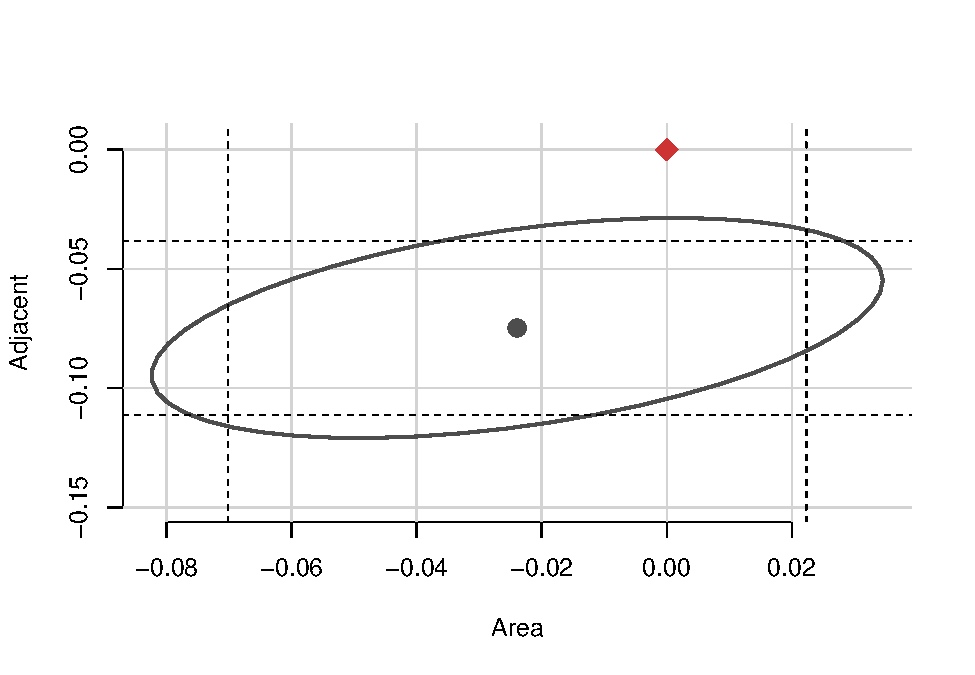
\includegraphics[width=0.8\linewidth]{Lab_6_files/figure-latex/unnamed-chunk-24-1} \end{center}

Cum punctul \((0,0)\) nu aparține regiunii elipsoidale atunci putem
respinge ipoteza nulă \(H_0:\beta_{Area}=\beta_{Adjacent}=0\).

\renewcommand\refname{Referințe}
\bibliography{references/InstStatFin2018ref.bib}


\end{document}
